\documentclass[10pt, a4paper, spanish]{article}
\usepackage[paper=a4paper, left=1.5cm, right=1.5cm, bottom=1.5cm, top=3.5cm]{geometry}
\usepackage[utf8]{inputenc}
\usepackage[spanish,es-nodecimaldot]{babel}
\usepackage{caratula}
\usepackage[pdfencoding=auto, colorlinks=true, linkcolor=blue]{hyperref}
\usepackage[boxruled, longend]{algorithm2e}
\usepackage{wrapfig}
% \usepackage{tikz}
\usepackage[rightcaption]{sidecap}
% \usetikzlibrary{babel}
\usepackage{float}
\graphicspath{ {imagenes/} }

% \tikzset{nodeList/.style={every node/.style={draw, circle}}}
% \tikzset{pathList/.style={every node/.style={midway, fill=white}}}


\newcommand{\ord}{\ensuremath{\operatorname{O}}}
\newcommand{\nat}{\ensuremath{\mathbb{N}}}

\begin{document}
% CARATULA
\materia{Métodos Numéricos}
\submateria{Primer Cuatrimestre de 2018}
\fecha{\today}
\grupo{Los arboles mueren de pie}
\titulo{Trabajo Práctico 2}

\integrante{Giudice, Carlos}{694/15}{carlosr.giudice@gmail.com}
\integrante{Szperling, }{763/15}{juanju@dc.uba.ar}

\maketitle

\newpage
\tableofcontents

\newpage
\section{Introducción}

Este trabajo práctico tiene como objetivo el desarrollo y estudio de una herramienta que permita reconocer dígitos manuscritos en imágenes. El algoritmo capaz de llevar esto a cabo es uno de clasificación supervisado que fue entrenado con un lote de caracteres conocido, de modo que le sea posible reconocer otras instancias de esos caracteres aprendidos que no se encuentren en la base de datos de entrenamiento.

En cuanto al reconocimiento de dígitos, estos serán entre el 0 y el 9, y estarán plasmados en imágenes en escalas de grises.

\subsection{Evaluación}

Para el estudio de esta herramienta es necesaria la evaluación de los métodos y la correcta elección de sus parámetros. Una forma de evaluación es la estimación de la correctitud de la clasificación, para lo cual es necesita conocer previamente a qué dígito corresponde cada imagen. La forma de realizar esto es particionar la base de entrenamiento en dos, utilizando una parte de ella en forma completa para el entrenamiento y la restante como test, pudiendo así corroborar la clasificación realizada, al contar con el etiquetado del entrenamiento.

Sin embargo, realizar toda la experimentación sobre una única partición de la base podría resultar en una incorrecta estimación de parámetros, como por ejemplo el conocido caso de overfitting. Por lo tanto, se implementó la técnica de \textit{K-fold cross validation} que resulta estadísticamente más robusta.

El resultado del algoritmo final fue medido con distintas métricas (Accuracy, Curvas de precisión/recall).

% ____________A CORREGIR_______________
% 1 - Tiempos gramaticales
% 2 - Introduccion Teorida? (Lo puso Nestor)


\newpage
\section{Desarrollo}

\subsection{kNN}

El algorimo kNN (k Nearest Neighbours) se basa en el análisis de un conjunto de puntos del espacio para determinar a qué clase corresponde el nuevo objeto. En este caso cada imagen estará representada como un vector donde cada elemento es un píxel distinto de la misma. El conjunto de puntos elegido serán aquellas $k$ imágenes que más cerca se encuentren de la imagen a clasificar. Se clasificará a la nueva imagen como perteneciente a la clase que mayor representantes tenga en este conjunto de puntos cercanos.

Este algoritmo puede ser sumamente costoso en cuanto al tiempo de cómputo, y si la dimensión de los puntos a clasificar es muy grande, hacer uso del mismo podría resultar impracticable. Es por esto que se implementó un método cuyo objetivo es preprocesar las imágenes para reducir la cantidad de dimensiones de las muestras, permitiendo a kNN trabajar con muestras de una menor cantidad de variables. Este método es conocido como PCA (Principal components analysis).

\subsection{PCA}

El método de análisis de componentes principales se encarga de cambiar de base el conjunto de datos de entrada para obtener una mejor representación de los datos, y además reduce la dimensión de cada elemento tanto como se desee. Al reducir la dimensión de un punto es claro que se pierde información sobre el mismo, pero la particularidad de este método es que, se queda con las componentes más importantes, dejando de lado las que menos información aporten (de allí su nombre). De este modo, la información que descartada es la de menor relevancia, por lo que se lo considera una buena manera de reducir el espacio de la entrada.

Es importante aclarar que el método no solamente reduce la dimensión de los datos, sino que cambia la base de los mismos. Si se utiliza el método para reducir la entrada de kNN, es necesario cambiar a la misma base la imagen a clasificar, de lo contrario estarían comparándose elementos pertenecientes a distintos espacios.

\bigskip

Procedimiento para el cambio de base:

\begin{enumerate}
\item Se define una base de datos de entrenamiento (para $kNN$) como el conjunto $\D = \{x_i : i = 1, . . . , n\}$.
\item Sea $\mu = (x_1 + ... + x_n)/n$ el promedio de las imágenes de $D = \{x_i : i = 1, ..., n\}$ tal que $x_i\in\mathbb{R}^{m}$. Definimos $X\in\mathbb{R}^{nxm}$ como la matriz que contiene en la $i$-ésima fila al vector $(x_i - \mu)^t/  \sqrt{n-1}$. La matriz de covarianza de la muestra $X$ se define como $M = X^t X$
\item Se calcula $X$ y con ella $M$.
\item Se calculan los autovectores de $M$ mediante el método de las potencias, con deflación. Cómo cada iteración en la que calculamos el autovector de la matriz en cuestión, este está asociado al autovalor de máximo módulo, los autovectores que habremos calculado se encontrarán ordenados por relevancia. De esta manera se calculan tan solo $\alpha$ autovectores, con $1 \leq \alpha \leq n$, siendo $\alpha$ la dimensión a la que se quiere reducir las imágenes. 
\item Se contruye la matriz $V$ con los autovectores calculados previamente, dispuestos como columnas. $V$ es la matriz de cambio de base.
\item Por último, se reduce la dimensión de $X$ cambiando su base. El resultado final es $V^tX^t$ que contiene la misma cantidad de imágenes pero expresadas en otra base, y en lugar de tener dimensión $n$, cada una tiene dimensión $\alpha$.
\end{enumerate}\tabularnewline

Es interesante notar que una vez hecho el cambio de base de las imágenes, éstas representan a las imágenes pero si se trata de graficarlas se obtendrá algo muy distinto a lo que era anteriormente y no podrá visualizarse nada en concreto. Solo volviendo a la base original sería posible, pero ya se habrá perdido mucha información por lo que probablemente sea difícil encontrarlo útil.

\subsection{Fotos y algorítmo Peola}

\begin{algorithm}[H]
\NoCaptionOfAlgo
	\KwData{	
	img, $\alpha$, $\sigma$ 
	\KwResult{La imagen manipulada}
	\caption{Deformación}
	\tcc{Generamos 2 matrices de desplazamiento aleatorias} 

	dx $\leftarrow$ rand(size(img))

	dy $\leftarrow$ rand(size(img))

	\tcc{Suavizamos con un filtro gausseano la aleatoriedad de la matriz}
	fdx $\leftarrow$ $\alpha *$ imgaussfilt(dx, $\sigma$)

	fdy $\leftarrow$ $\alpha *$ imgaussfilt(dy, $\sigma$)

	\tcc{Aplica el desplazamiento aleatorio usando la interpolacion de griddata}
	res $\leftarrow$ griddata(fdx, fdy, img)
		}
\end{algorithm}

\begin{figure}[!htb]
\minipage{0.32\textwidth}
  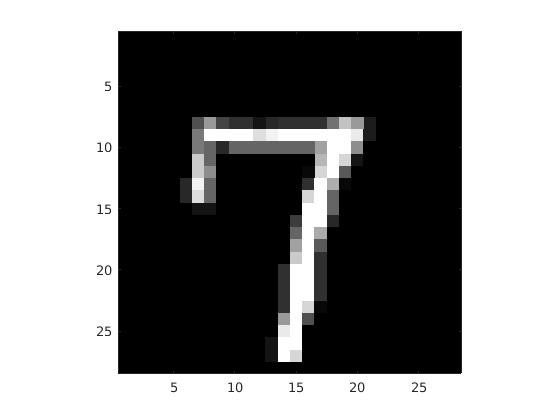
\includegraphics[width=\linewidth]{7original.jpg}
  \caption{Original}
\endminipage\hfill
\minipage{0.32\textwidth}
  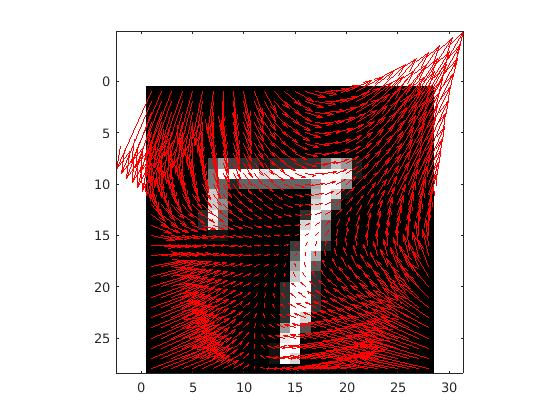
\includegraphics[width=\linewidth]{7vectpres.jpg}
  \caption{Vectores de desplazamiento}
\endminipage\hfill
\minipage{0.32\textwidth}%
  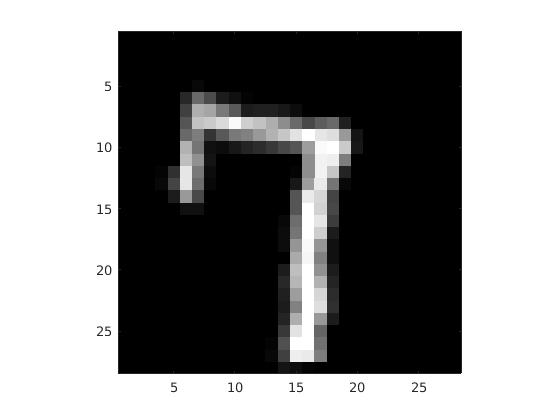
\includegraphics[width=\linewidth]{7resultado.jpg}
  \caption{Resultado}
\endminipage
\end{figure}


Como se puede observar, el dígito resultante es distinto al original pero al ojo humano sigue siendo el mismo dígito. Con este método generamos un nuevo data-set aplicando esta función a cada imagen y así ahora tenemos el doble de datos 84000 dígitos. 

Además de notar que los trazos no son perfectos, la orientación y rotación de los dígitos no es siempre la misma. Quisimos llevar al extremo aumentar los datos y aplicamos una segunda transformación a los dígitos. Para ello aplicamos una rotación aleatoria a cada dígito, usando la función de matlab para rotar imágenes imrotate, generamos un número aleatorio entre un cierto rango que le pasamos por parámetro como el ángulo. 30 grados nos pareció razonable ya que si se le aplica más hay dígitos que no se verían beneficiados.

\begin{figure}[ht] 
  \begin{minipage}[b]{0.5\linewidth}
    \centering
    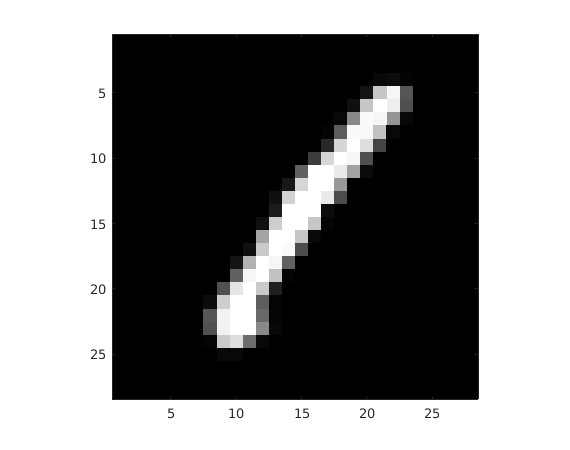
\includegraphics[width=.5\linewidth]{1_sinrotar.png} 
    \caption{Dígito Original 1} 
    \vspace{4ex}
  \end{minipage}%%
  \begin{minipage}[b]{0.5\linewidth}
    \centering
    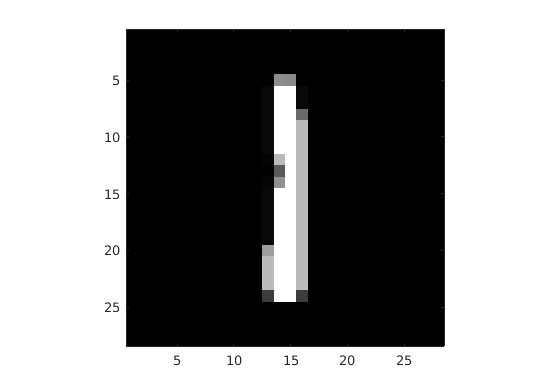
\includegraphics[width=.5\linewidth]{1_parecido.png} 
    \caption{Dígito Original 2} 
    \vspace{4ex}
  \end{minipage} 
  \begin{minipage}[b]{0.5\linewidth}
    \centering
    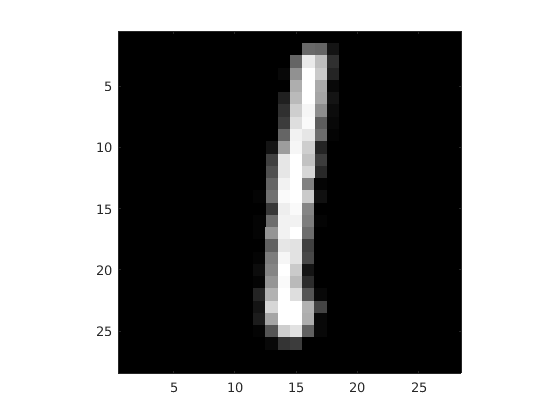
\includegraphics[width=.5\linewidth]{1_rot30.png} 
    \caption{Dígito 1 rotado $30^\circ$ sentido horario} 
    \vspace{4ex}
  \end{minipage}%% 
  \begin{minipage}[b]{0.5\linewidth}
    \centering
    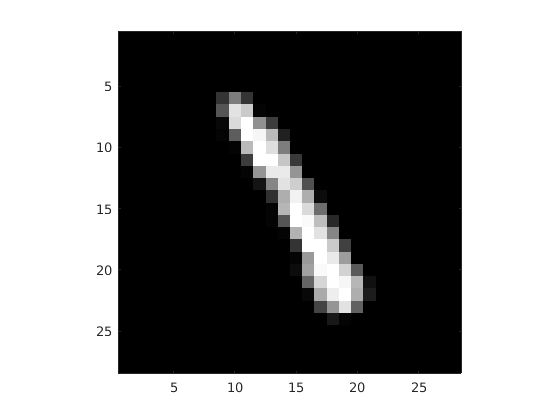
\includegraphics[width=.5\linewidth]{1_chueco.png} 
    \caption{Dígito 2 rotado $30^\circ$ sentido horario} 
    \vspace{4ex}
  \end{minipage} 
\end{figure}


\subsection{$X^t*X$ y $X*X^t$}
El método de la potencia con deflación se utiliza para obtener tanto los autovectores como los valores asociados de una matríz. Éste método es particualarmente suceptible al tamaño de la matríz que entra como parámetro. Al ser $X\in\mathbb{R}^{nxm}$ (con $m >> n$), la matríz $M$ acarrea un gran costo temporal para el cómputo del método de la potencia con deflación. Por lo que definimos la matríz $\^{M}\in\mathbb{R}^{nxn}$ como $\^{M}=X*X^t$. Como podemos ver, $\^{M}$ depende de la cantidad de imágenes de training set (que tiene como cota superior 410), por lo que será mucho más chica que $M$. Propondremos un método que utiliza los autovectores y autovalores de $\^{M}$ (cuyo cálculo implíca menor costo temporal) para obtener los de $M$.

\\
Primero veamos que relación hay entre los autovectores y los autovalores de {$X^t*X$ y $X*X^t$}:\\
\begin{center}
Sea $X\in\mathbb{R}^{nxm}$, $\^{M}=XX^t$ y $M=X^tX$.\\
Sea $v_i$ el autovector de $\^{M}$ asociado a $\lambda_i$, para  $i = 1, ..., n$.\\
\Rightarrow $\^{M}v_i=\lambda_iv_i$, para  $i = 1, ..., n$. Por definición de autovalor y autovector.\\
\Rightarrow $XX^tv_i=\lambda_iv_i$. Porque $\^{M}=XX^t$. \\
\Rightarrow $X^tXX^tv_i=\lambda_iX^tv_i$. Multiplico a izquierda por $X^t$.\\
 Defino $u_i=X^tv_i$\\
\Rightarrow $X^tXu_i=\lambda_iu_i$\\
Como $M=X^tX$,\\
\Rightarrow$Mu_i = \lambda_iu_i$\\
\therefore $u_i$ es el autovector de $M$ asociado al autovalor $\lambda_i$
\end{center}\\
\bigskip

Procedimiento para obtener los autovectores y autovalores de $M$ a partir de  $\^{M}$ utilizando la definición de $u_i$ que acabamos de formular:
\begin{enumerate}
\item Utilizando el método de la potencia con deflación se calculan los autovectores y autovalores de $\^{M}=X*X^t$ ($v_i$ y $\lambda_i$, para  $i = 1, ..., n$). 
\item Se crea una matríz $V\in\mathbb{R}^{nxn}$ y en sus columnas se colocan los autovectores $v_i$ de $\^{M}$ en el orden que fueron apareciendo (el método de la potencia con deflación devuelve los autovectores ordenados por módulo y sus autovectores correspondientes). Se guardan aparte los $n$ autovalores $\lambda_i$,  $i = 1, ..., n$.
\item Se calcúla $U=X^t*V$, en cada columna $U$ tendrá $u_i = X^t*v_i$ para $i = 1, ..., n$.
\item Recorriendo las columnas de $U$ se recuperan los autovectores $u_i$ de $M$.

\end{enumerate}\tabularnewline


\subsection{Validación cruzada}
Dado que necesitamos conocer previamente a qué persona corresponde una imagen para
poder estimar la correctitud de la clasificación, una alternativa es particionar la base de
entrenamiento en dos, utilizando una parte de ella en forma completa para el entrenamiento
y la restante como test, pudiendo ası́ corroborar la clasificación realizada, al contar con el
etiquetado del entrenamiento. Sin embargo, realizar toda la experimentación sobre una única
partición de la base podrı́a resultar en una incorrecta estimación de parámetros, dando lugar
al conocido problema de overfitting.\\
Por lo tanto, se estudiará la técnica de $cross validation$, en particular el $K-fold cross
validation 1$ , para realizar una estimación de los parámetros de los métodos que resulte estadı́sticamente más robusta.\\


La validación cruzada \textit{K-fold} consiste en particionar la base de entrenamiento en $K$ partes del mismo tamaño. Luego se realiza $K$ iteraciones, cada una de ellas reteniendo uno de los conjuntos para validación y utilizando los restantes $K - 1s$ para entrenamiento. Este método usualmente permite tomar las particiones sin cuidado alguno, pero en nuestro caso de uso tal cosa no es conveniente. Esto se debe a que en nuestra base de entrenamiento cada persona está representada por diez imágenes, con lo cual dividir las muestras de forma aleatoria puede desbalancear que tan representadas estan algunas personas en el training set. Esto puede significar que el algoritmo se entrena poco para algunas personas y mucho para otras. Yendo más lejos, este desbalance en el train set siempre tiene su contraparte en el test set, impactando de forma negativa las métricas.
Para resolver este problema, se propuso el uso de un k-fold que respete las proporciones de imágenes de cada persona. Como el test set siempre tiene que tener la misma cantidad de fotos para cada persona. Como nuestro dataset cuenta con cuarenta y un personas diferentes, la cantidad de rows del test set será un multiplo de ese número. Esto implica que k será multiplo de diez. Se realizó un shuffle de las imágenes y se eligieron los folds respetando las proporciones mencionadas.



\newpage
\section{Resultados}

Uno de los objetivos de la experimentación de este trabajo era encontrar los mejores parámetros para los métodos, es decir, los parámetros para los cuales los algoritmos proporcionaban mejores resultados. Para determinar la calidad de los resultados obtenidos (cuáles eran los mejores) se tuvo en cuenta distintas métricas, que ayudaron a determinar esto mismo:

\begin{itemize}
\item Accuracy
\item F1-Score
\end{itemize}

Los resultados obtenidos fueron analizados en términos de estas métricas aplicando validación cruzada \textit{K-fold}, variando el $K$ sobre la base de entrenamiento.

Los parámetros $k$ (cantidad de vecinos en \textit{kNN}, no confundir con $K$ de \textit{K-fold}) y $\alpha$ (dimensión a la cual se reduce cada imagen con \textit{PCA}) fueron variándose como se expondrá en las páginas siguientes.

Además de las métricas mencionadas, se tuvo en cuenta el tiempo de computo para las distintas entradas.

\subsection{Tiempo de ejecución Knn}

Dado que el costo temporal de knn no depende del parámetro k, lo que nos interesa es entender el costo fijo por predicción. En un dataset de 205 imágenes reducidas, el costo promedio de clasificación de una imágen fue de 0.00042. Comparamos ese resultado con el costo promedio para la misma cantidad de imágenes de tamaño completo y el resultado fue 0.11738, varios órdenes de magnitud mayor. 

\subsection{Tiempo de ejecución PCA+Knn}

Para evaluar el costo temporal de las predicciones de Knn al utilizar PCA, es necesario tener en cuenta el costo de la transformación característica, que se realiza a cada imágen a predecir para poder compararla con las imágenes de entrenamiento transformadas gracias al PCA. Otro factor a tener en cuenta es que el alpha de PCA define la dimensión de las imágenes que compara el Knn, esto impacta directamente a la cantidad de operaciones necesarias y consecuentemente al tiempo de cómputo.

\begin{figure}[H]
	\begin{center}
      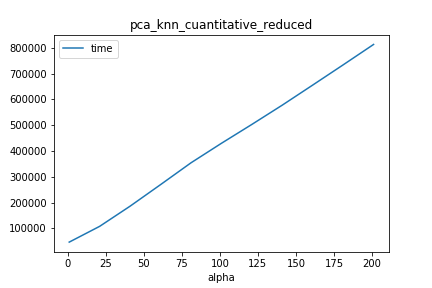
\includegraphics[width=0.4\columnwidth]{imagenes/charuli-des/pca_knn_cuantitative_reduced.png}
      \caption{Costo temporal de tc + predicción de knn}
      \end{center}
\end{figure}

\subsection{Tiempo de ejecución PCA}

Con el objetivo de entender el costo de calcular una matriz de covarianzas para una muestra X, probamos con diferentes cantidades de imagenes reducidas y con diferentes valores del alfa de PCA. 

Para visualizar los resultados de los experimentos para cada X, se creó un gráfico donde la variable independiente es el alpha y la variable dependiente es el tiempo de cómputo. 

En los gráficos Observamos que el tiempo de cómputo se comporta de forma lineal en ralción al alpha para distintos segmentos de alpha, pero la pendiente es discontinua.

\begin{figure}[H]
	\begin{center}
      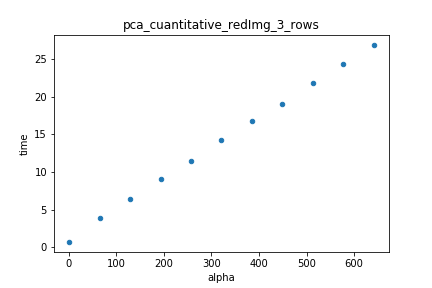
\includegraphics[width=0.4\columnwidth]{imagenes/charuli-des/pca_cuantitative_redImg_3_rows.png}
      \caption{Costo temporal de PCA para tres imágenes reducidas}
      \end{center}
\end{figure}
\begin{figure}
	\begin{center}
    	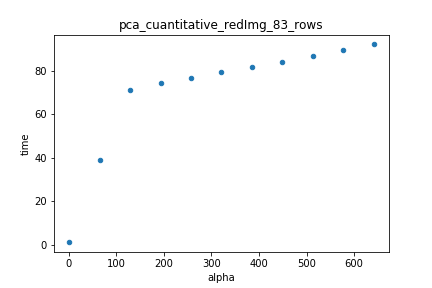
\includegraphics[width=0.4\columnwidth]{imagenes/charuli-des/pca_cuantitative_redImg_83_rows.png}
     \caption{Costo temporal de PCA para ochenta y tres imágenes reducidas}
     \end{center}
\end{figure}

\subsection{Tiempo de ejecución}

Medimos 2 cosas en términos de los tiempos de ejecución: el tiempo que toma realizar PCA sobre el set de entrenamiento, y el tiempo en aplicar kNN sobre uno de los elementos (incluyendo el cambio de base en el caso de haber realizado PCA).

Para estas mediciones tomamos los sets de entrenamiento y prueba provistos por la cátedra, correspondientes a la competencia de Kaggle. También usamos para estas pruebas $k = 10$ (para kNN) y $alpha = 100$ (para PCA). 

Los resultados fueron que, para el caso sin PCA, cada elemento de prueba tarda en promedio 500 ms en ser procesado. Consideramos que esto es relativamente lento, ya que al tratarse de 28,000 elementos, esto suma en total 3.89 horas, lo que resulta bastante prohibitivo y fue problemático a la hora de hacer experimentaciones.

En contraste, en el caso con PCA, cada elemento era procesado en aproximadamente 95ms, una mejora sustancial sobre todo considerando que esto incluye el cambio de base. Al aplicar sobre el set de prueba completo, esto demora alrededor de 45 minutos, una fracción del tiempo mencionado anteriormente.

Por último, cabe destacar que PCA en sí es un proceso costoso. Sin embargo, como nos esperábamos, el costo de PCA está compensado por las dimensiones de los sets utilizados, y aplicarlo sobre nuestro conjunto de entrenamiento demora en promedio 26 minutos, por lo que sumado a kNN, sigue representando apenas más del 25\% del tiempo de ejecución sin PCA.

Sin embargo, debe recordarse que el costo de PCA es elevado. Esto debe tenerse en cuenta junto con la precisión obtenida para sets de datos más pequeños, ya que podría no justificarse.

\subsection{K de kNN}

Utilizamos las imagenes de tamaño completo, sin transformaciones. Llamamos k a la constante que define cuantos vecinos se tienen en cuenta a la hora de decidir la categoría de la muestra a clasificar. Los valores probados para k fueron 1, 3, 8, 10, 15 y 25. Se observó consistentemente que todas las métricas decrecen a medida que se incrementa el valor de k. Siendo $k = 1$ el valor óptimo. 

\begin{figure}[H]
    \begin{center}
      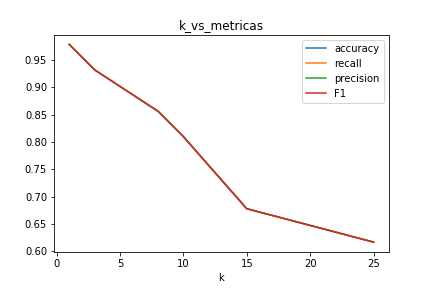
\includegraphics[width=0.8\columnwidth]{imagenes/charuli-des/k_vs_metricas.png}
      \caption{Metricas para distintos valores de k}
    \end{center}
\end{figure}

La diferencia en la calidad de las predicciones tambien puede observarse  visualizando matrices de confusión.

\begin{figure}[H]
    \begin{center}
      \includegraphics[width=0.8\columnwidth]{imagenes/charuli-des/Confusion_matrix_for_k_1.png}
      \caption{Metricas para distintos valores de k}
    \end{center}
\end{figure}

\begin{figure}[H]
    \begin{center}
      \includegraphics[width=0.8\columnwidth]{imagenes/charuli-des/Confusion_matrix_for_k_25.png}
      \caption{Metricas para distintos valores de k}
    \end{center}
\end{figure}

\subsection{K de kNN old}

Para analizar el comportamiento al cambiar el K de kNN fijamos alpha de PCA en 2 valores 15 y 30. Corrimos experimentos para distintos estos K: 1, 2, 3, 4, 5, 7, 8, 8, 10, 15, 20, 30.

Nuestra hipótesis previo a correr los experimentos fue que para $k$s chicos, la posibilidad de que nuestro vecino más cercano sea un outlier representando otro dígito son más altas y para los $k$s grandes, pensamos que los dígitos que se encuentran en las fronteras, osea que se parecen a otros dígitos, se verían perjudicadas ya que por como funciona knn, pordía ocurrir que el más cercano sea, por ejemplo, 5 pero todos los siguientes sean 2. Por lo tanto, supusimos que los $k$s intermedios serían los que mejor funcionarían.

Habiendo corrido los experimentos, el gráfico de accuracy generado fue el siguiente:

\begin{figure}[H]
    \begin{center}
      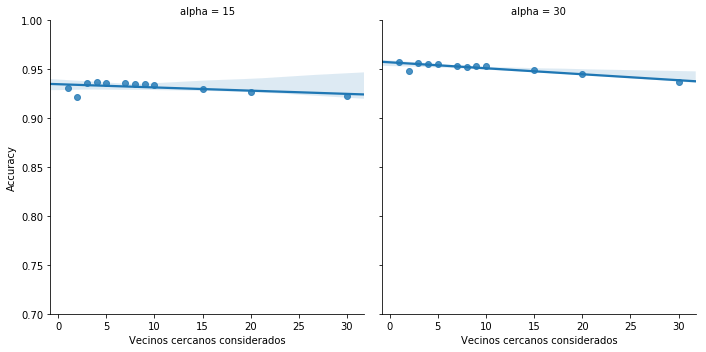
\includegraphics[width=0.8\columnwidth]{imagenes/Accuracy_15_30.png}
      \caption{Accuracy por k de kNN con alfa de PCA fijo}
    \end{center}
\end{figure}

Lo que se observó en este gráfico fue que el algoritmo es estable para los distintos $k$s y que las diferencias fueron poco significativas, pero pudimos contrastar con la hipótesis que lo que propusimos estaba en lo correcto.

El siguiente gráfico es una comparación del F1 score sobre los mismos resultados anteriores.

\begin{figure}[H]
    \begin{center}
      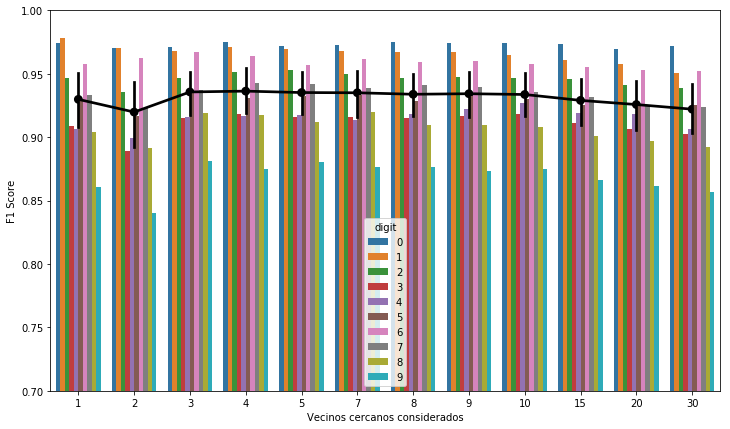
\includegraphics[width=0.8\columnwidth]{imagenes/F1_alpha_15.png}
      \caption{F1 score por k de kNN con alfa de PCA fijo en 15}
    \end{center}
\end{figure}

\begin{figure}[H]
    \begin{center}
      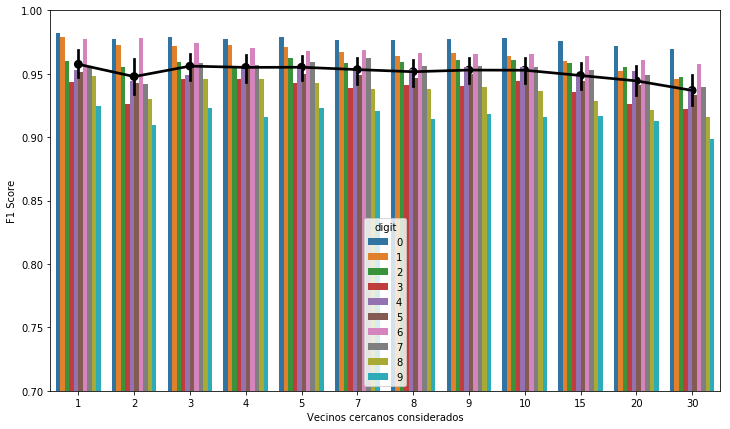
\includegraphics[width=0.8\columnwidth]{imagenes/F1_alpha_30.png}
      \caption{F1 score por k de kNN con alfa de PCA fijo en 30}
    \end{center}
\end{figure}

Este gráfico nos mostró también que el algoritmo es estable para cada dígito y que para alfa 30 de PCA las diferencias entre los dígitos es menor. En la siguiente sección entraremos en detalle sobre la comparación que realizamos sobre el alfa de PCA.

\subsection{Alfa de PCA}

El otro parámetro que tratamos de optimizar fue el alfa de PCA, de una forma similar al K, fijamos este y fuimos cambiando el alfa, por suerte ya teníamos resultados sobre el K, así que decidimos fijarlo en 5. Los alfas con los que experimentamos fueron: 5, 10, 15, 20, 25, 30, 40, 50, 60, 80, 100, 150

Nuestra hipótesis para este experimento fue que si tomabamos un alfa bajo tendríamos bastante ruido y que para alfas grandes, al agregar tantas componentes, se daría menor importancia a los componentes mas relevantes por lo que perdería un poco de calidad de resultados ya que utilizar valores altos tiende a parecerse a sólo hacer kNN.

El siguiente gráfico muestra el accuracy para cada alfa evaluado.

\begin{figure}[H]
    \begin{center}
      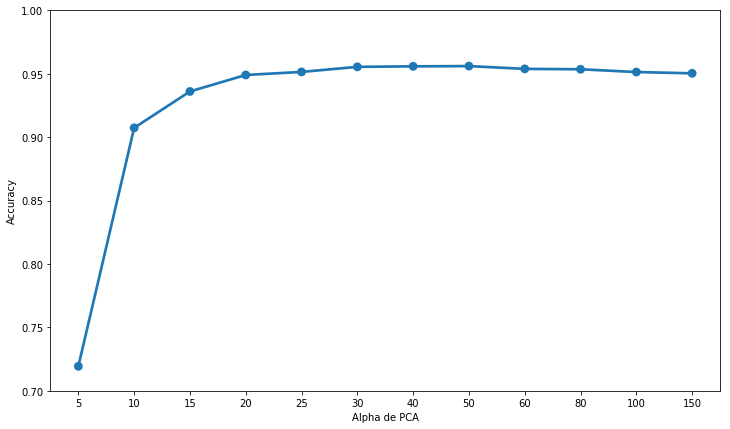
\includegraphics[width=0.8\columnwidth]{imagenes/Accuracy_all_alpha.png}
      \caption{Accuracy por alfa de PCA con k de kNN fijo en 5}
    \end{center}
\end{figure}

En este gráfico pudimos ver que los alfas que mejor funcionan de acuerdo al accuracy son los alfas entre 30 y 50 ya que a partir de ese momento es cuando el accuracy (lentamente) empieza a bajar.

El siguiente gráfico muestra F1 por dígito para cada alfa evaluado.

\begin{figure}[H]
    \begin{center}
      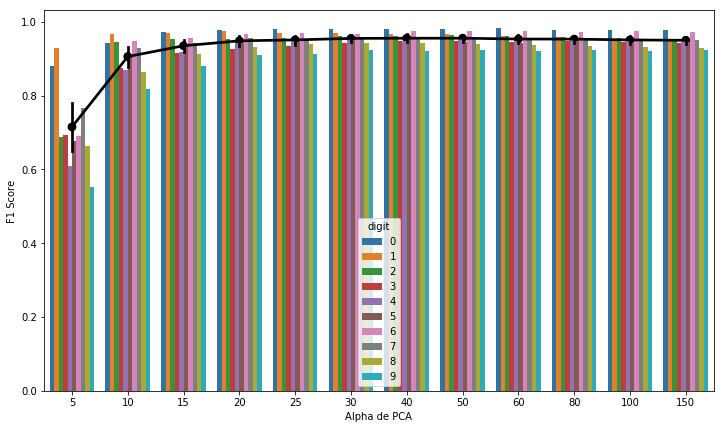
\includegraphics[width=0.8\columnwidth]{imagenes/F1_per_digit.png}
      \caption{F1 score por alfa de PCA con k de kNN fijo en 5}
    \end{center}
\end{figure}

En este caso se observó que para alfas muy bajos los resultados fueron bastante peores y que a medida que crece el alfa, se estabilizan más los resultados. 
Sabemos que a mayor alfa, más lento anda el algoritmo, por lo que podemos concluir que no es bueno tomar este tipo de valores dada la pequeña diferencia de calidad que hay entre ellos. Por eso decidimos que 30 era un buen alfa.

En base a estos experimentos concluímos que nuestra hipótesis era correcta, aunque esperábamos que para valores como 150 ande peor que lo que realmente funciona.

\subsection{Data augmentation}

Antes de entrenar el algoritmo con todo el dataset quisimos ver cómo el modelo de transformaciones escalaba, para eso corrimos sobre un subconjunto del set de datos, a los mismos 10k digitos les aplicamos la transformación para obtener así un dataset de 20k. Como ya teníamos el K y el alfa analizados usamos 5 y 30 respectivamente. Los resultados del experimento fueron una accuracy de 0.9602 para las rotaciones y de 0.9715 para las deformaciones elásticas. Pudimos apreciar una gran mejora con las deformaciones elásticas, esto se puede deber a que las rotaciones hay casos en los que no queda tan real el dígito generado.


\newpage
\section{Conclusiones}

En base a lo explicado en las secciones anteriores de este trabajo, pudimos concluir que los valores que mejor funcionan para nuestro algoritmo son 5 para kNN y 30 para el alfa de PCA. Más aún, podemos decir con confianza que el uso de análisis de componentes principales mejoró la calidad y el tiempo de ejecución de forma drástica para el set de datos provisto. No obstante, para que esto funcione de forma óptima se necesita un set de datos amplio como el utilizado para este trabajo. Además, encontramos que el método tiene un límite de precisión que no pudimos superar a pesar de realizar distintas técnicas y experimentaciones, si bien el mismo es elevado (casi 98\% de Accuracy).

En resumen, consideramos que este algoritmo es muy útil en casos donde una exactitud del $100\%$ no es indispensable, dada la calidad de los resultados y su sencilla implementación. Hacemos esta aclaración ya que este mismo algoritmo puede ser y es comunmente utilizado para múltiples problemas de clasificación, donde los datos de entrada son multidimensionales.


\newpage
\section{Apéndice}

\subsection{Apéndice I: detalles de implementación}

Para poder soportar la posible necesidad de matrices más eficientes en memoria, creamos una clase Matrix con múltiples implementaciones. La misma tiene métodos para cada operación que consideramos necesaria, y algunas otras utilidades que utilizamos en el Trabajo Práctico 1. Por otro lado, implementamos una matriz completa (con vectores de la biblioteca estándar de C++), una matriz dispersa (usando mapas), y otras versiones más específicas.

Para evitar complicaciones con el manejo de punteros y el polimorfismo, utilizamos \texttt{std::shared\_ptr} de C++11, que se encarga de borrar las matrices que no necesitamos por nosotros.

Sin embargo, luego nos dimos cuenta que los casos de uso de este TP no requieren varias versiones especificas como si las requería tal vez el TP anterior. La implementación sigue incluída, pero solo se usa la versión completa de la matriz (denominada \texttt{FullMatrix}).

Otro elemento que dejamos en la implementación pero no se utiliza fueron unos pseudo-iteradores para las imágenes que recorren archivos en lugar de vectores en memoria. El mismo no se usa porque es muy poco eficiente (ya que lee múltiples veces un archivo en disco), y luego de medir el consumo de memoria lo consideramos innecesario.

Por otro lado, decidimos abstraer el entrenamiento y el reconocimiento de las imágenes en una clase común, a modo de intercambiar implemetaciones rápidamente y por parámetros. Hoy en día nuestro TP solo cuenta con 2 implementaciones: kNN y kNN + PCA, pero podrían argegarse otras variaciones a futuro.

\subsection{Apéndice II: código complementario en MATLAB}

Además del código con el reconocimiento de dígitos implementado en C++, incluímos en la entrega algunos scripts de MATLAB que nos resultaron útiles durante la experimentación. Los mismos incluyen comentarios explicando su funcionalidad, pero todos están relacionados a los datos con los que expermientamos (con algunos métodos para probar incrementando el set de entrenamiento) y los resultados de dichos experimentos (validación cruzada, F1 score, etc).


% compilar 2 veces para actualizar las referencias


\end{document}